%!TEX root = Main.tex
\section{Results}

\subsection{Proof-of-Concept prototype}

The outcome of this study was a prototype, able to send messages from both a Shimmer unit and a CareBed to a service, as seen on Figure \ref{fig:deployment}.
The service could transfer the data from their respective data types to a shared data structure to be stored with a recalculated probability of the event occurring.
The service is capable of being plugged into the CAALHP without changing anything within the framework, and provides storage of all occurred events (structure seen on Figure \ref{fig:UML}) and all latest event from each sensor.

\begin{figure}[hbtp]
	\centering
	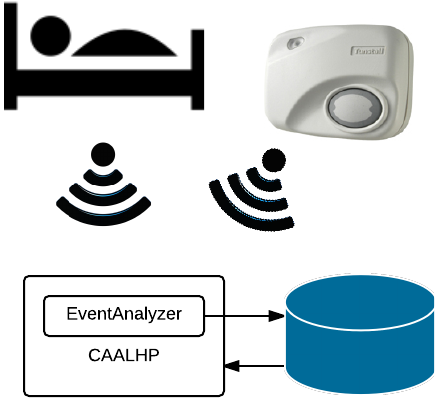
\includegraphics[width = 0.40 \textwidth]{Deployment}
	\caption{Deployment diagram of the system. 
		Each sensor is connected to the CAALHP with a wireless link.
		Inside the CAALHP runs the analyzer module with the false-positive filter in.}
	\label{fig:deployment}
\end{figure}

\begin{figure}[hbtp]
	\centering
	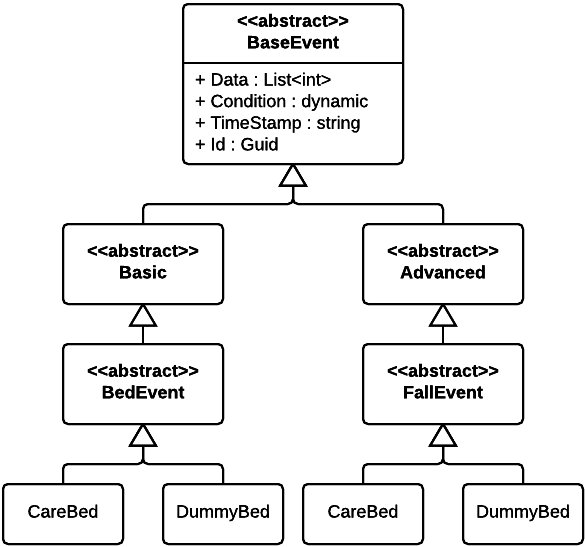
\includegraphics[width = 0.48 \textwidth]{UML}
	\caption{UML diagram of the event classes.}
	\label{fig:UML}
\end{figure}




\subsection{Evaluation}

The program consist of 27 tests, all green, varying from unit testing inserting new elements in the databases, to integration testing calculations of new, incomming events and whether they are stored with correct values.

Besides that is several tests of activating the Shimmer unit tested, while sitting and not sitting in the Carebed, which all gives expected results of the likelyhood of the Shimmer being false-positive or not.



\subsection{Sensor recommendation}

Of the different sensors, some of them works in similar ways, but not all with open APIs.
If a sensor does not have a open API to be used, the CAALHP cannot use them and they are not recommended.

Therefore Tunstall's product line, and the Yes Group is the only companies which can be recommended for this system.

MariCare's intelligent floor holds value regular PIR sensors can't provide, in form of detecting sudden pressure evenly spread, instead of a lot of pressure on two smaller areas.
It should only be considered, if a new floor is being laid out, and they open their API.

AnyGroup's API is not open yet, but they thought it might be at the end of the year 2015.
They have some products, all very easy to install, and non of them looks expensive.
AnyGroup's products are worth considering when their API gets opened.